\section{Day 3: Homeomorphisms and Bases (Sep. 10, 2024)}
Outfit of the day (by popular request)
\begin{figure}[h]
    \centering
    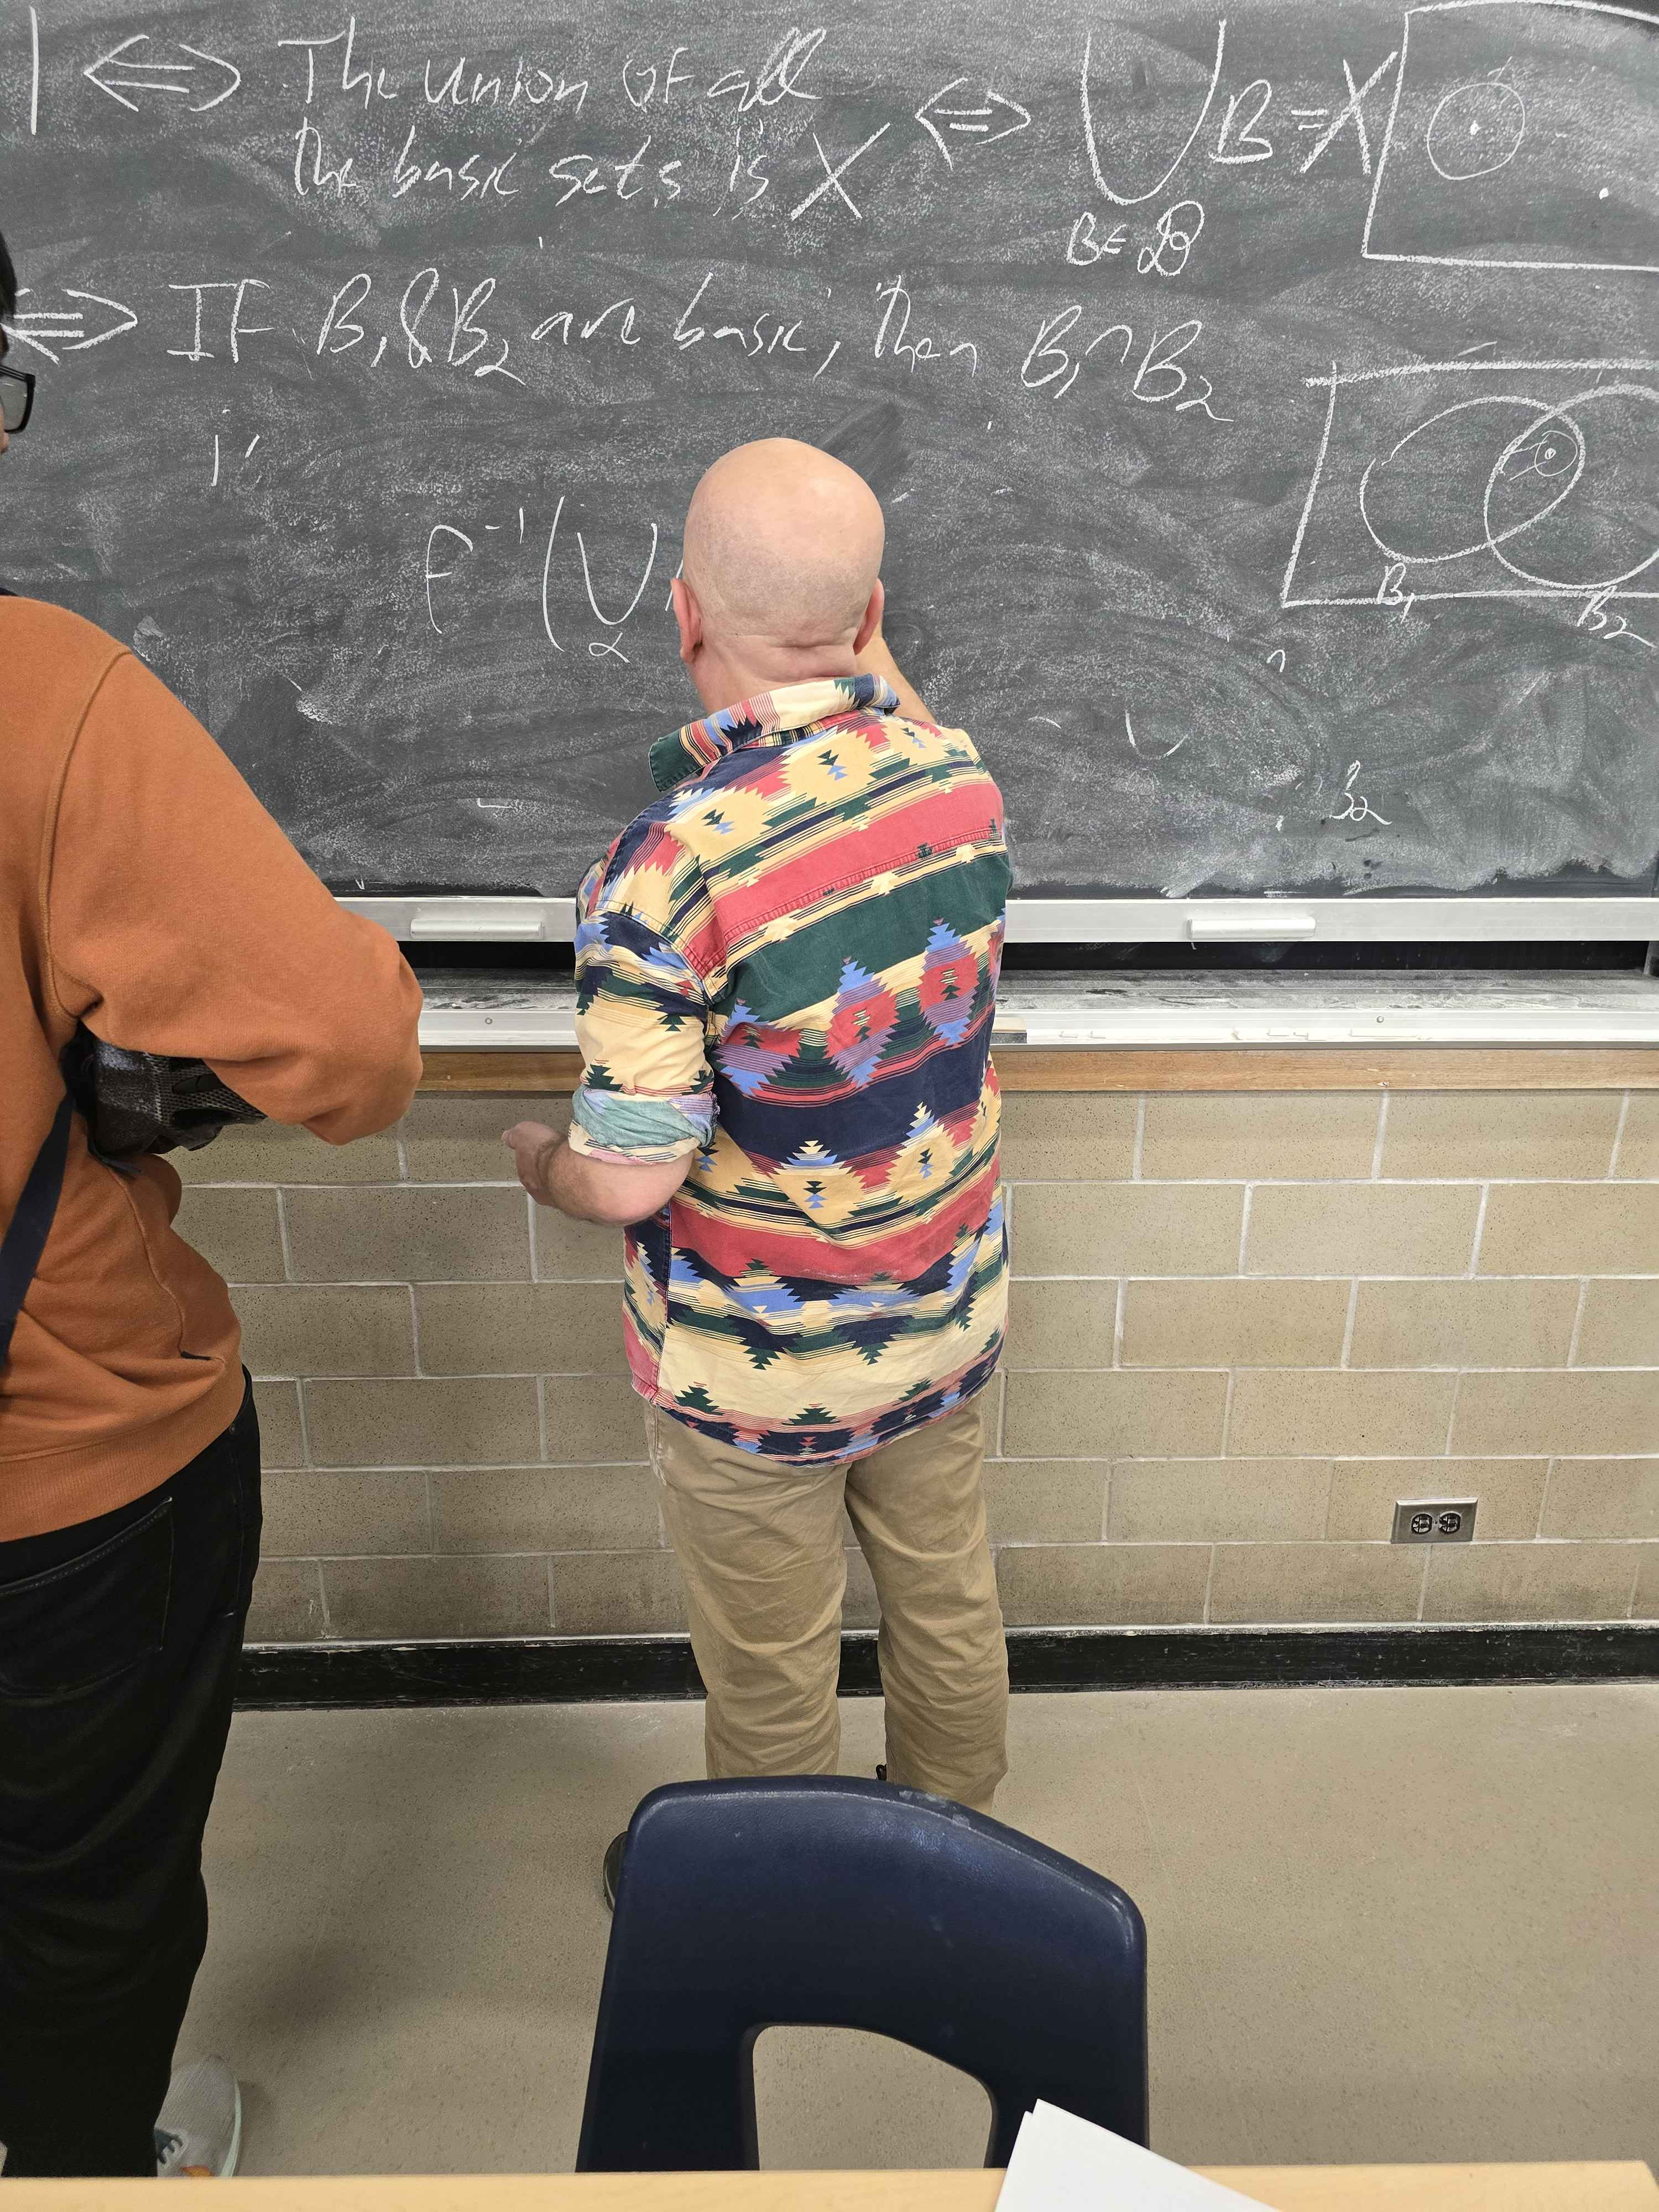
\includegraphics[scale=0.1]{MAT327 Notes/Dror Shirts/dror day 3 shirt.jpg}
\end{figure}

\noindent Course administrative details first;
\begin{itemize}
    \item The reading for this week is on sections $12$ to $14$ (this week will cover these contents), and $15$ to $16$ as prereading.
\end{itemize}
Recap of last lecture:
\begin{itemize}
    \item A topology $\ST \subset \SP(X)$ is a collection of subsets of $X$, of which we require $\{\emptyset, X\} \subset \ST$. We also require $\ST$ to be closed under arbitrary unions and finite intersections.
    \item We say a function $F : X \to Y$ is continuous if and only if for all $U \in \ST_Y$, we have $f^{-1}(U) \in \ST_X$.
\end{itemize}
Today we will cover homeomorphisms and bases. To start, recall the example topologies, such as $\ST_{\mathrm{std}}$ on $\RR^n$ (where $\ST_{\mathrm{std}}$ consists of the open balls), $\ST_\mathrm{triv}$, and $\ST_\mathrm{disc}$. We also introduce a new example topology (where FC standards for finite complement),
\[ \ST_\mathrm{FC} = \{ U \subset X \mid X \setminus U \text{ is finite, or } U = \emptyset \}. \]
Note that Prof. Bar-Natan may interchange the notations $-$ or $\setminus$ to represent set difference.
\begin{simplethm}[Composition of Continuous Functions is Continuous]
    Let $f : X \to Y$ and $g : Y \to Z$ be continuous functions. Then $g \circ f : X \to Z$ is continuous (relative to the same topologies on $X$ and $Z$).
\end{simplethm}
\noindent If $U \in \ST_Z$, we have $(g \circ f)^{-1}(U) = f^{-1} \circ g^{-1} (U)$, where by definition of continuity, we see that pre-images of open sets are open, and we have $g^{-1}(U)$ is open in $Y$, and similarly $f^{-1} (g^{-1}(U))$ is also open in $X$. \qed
\medskip\newline
\noindent In tutorial, we equipped $X$ with topologies $\ST_1, \ST_2$ (i.e., $X$ is a topological space in two ways). We say $\ST_1$ is finer than $\ST_2$ if $T_1 \supset T_2$, and coarser for the opposite direction; the words bigger and stronger may be used interchangeably with finer, and smaller or weaker for coarser. For example, the identity map
\[ \mathrm{id} : (X, \ST_1) \to (X, \ST_2) \]
is continuous if and only if $\ST_1$ is finer than $\ST_2$. To see this, let $U$ be an open set in $(X, \ST_2)$; then $U$ must be open in $(X, \ST_1)$ as well, which is true for any $U$ only if $\ST_1 \supset \ST_2$\footnote{includes the case $\ST_1 = \ST_2$; i'm following florian notation here with $\subset$ and $\subsetneq$ for explicit non equality}.
\begin{definition}[Homeomorphism]
    A map $h : X \to Y$ is called a homeomorphism if $h$ is continuous, bijective, and $h^{-1}$ is continuous as well.\footnote{smth smth coffee cup and donut ``extra homework: go find a nice video on why this is true on youtube''}
\end{definition}
\noindent Note that continuous bijective maps $h$ need not have continuous inverses; for example, let us have $\mathrm{id} : X_\mathrm{disc} \to X_\mathrm{triv}$. $\mathrm{id}$ is continuous as per our above example, while its inverse is not. Another example is to consider $[0, 2\pi) \to S^1$ (unit circle), where $x \mapsto (\cos 2x\pi, \sin 2x\pi)$; we see that the inverse is discontinuous at $0$ and $2\pi$ radians, even if the map is continuous and bijective (also observe that $[0, 1)$ is not compact while $S^1$ is).

\noindent An example of a homeomorphism is as follows (as per tutorial); let us consider\footnote{dror was using $\sim$ for homeomorphism symbol today. if he keeps using that i'll adjust my notes, but for now i'll use $\cong$ cuz afaik its used more...?}
\[ (-1, 1)_\mathrm{std} \cong \left(-\frac{\pi}{2}, \frac{\pi}{2}\right)_\mathrm{std} \cong \RR_\mathrm{std}, \]
where we may map the first to the second by $x \mapsto \frac{\pi}{2}x$, and the second to third by $x \mapsto \tan x$. Since the composition of continuous maps is continuous, we also see $(-1, 1)_\mathrm{std}$ is homeomorphic to $\RR_\mathrm{std}$ (any open interval is homophobic to $\RR$ for that matter).
\medskip\newline
\noindent Another example of a homemorphism is $\mathrm{id} : (X, \ST_1) \to (X, \ST_2)$ if $\ST_1 = \ST_2$.
\bigskip\hrule\bigskip
\noindent A ``basis'' for a topology on $X$ is a collection $\SB \subset \SP(X)$ of subsets such that
\begin{enumerate}
    \item For all $x \in X$, there exists some $B \in \SB$ such that $x \in B$. We call $B$ a \textit{basic set}.
    \item For all $B_1, B_2 \in \SB$ and $x \in B_1 \cap B_2$, there exists a third basic set $B_3$ such that $x \in B_3 \subset B_1 \cap B_2$.
\end{enumerate}

\newpage
\noindent In particular, the first condition is equivalent to $\bigcup_{B \in \SB} B = X$ (i.e., the basis forms a covering of $X$), and the second condition is equivalent to the basic sets contained in $B_1 \cap B_2$ forming a cover of $B_1 \cap B_2$, i.e.
\[ B_1 \cap B_2 = \bigcup_{\substack{B \in \SB \\ B \subset B_1 \cap B_2}} B. \]
Here are some examples;
\begin{enumerate}[label=(\alph*)]
    \item $\{B_r(x_0)\} \subset \SP(\RR^n)$, i.e. the open balls on $\RR^n$ form a basis.
    \item The one-dimensional analogue of case (a) is $\{(a, b) \mid a < b\}$, and it forms a basis on $\RR$.
    \item $\{[a, b) \mid a < b\}$ is called the lower limit topology, and it forms a basis on $\RR$.
    \item $\{[a, b] \mid a < b\}$ implies $[a, b] \cap [b, c] = \{b\}$, which forces the basic set to include all singletons on $\RR$. In that case, this is simply the discrete topology (?).
\end{enumerate}
\begin{simplethm}
    $\ST_\SB = \{ U \subset X \mid \forall x \in U \implies \exists B \in \SB \text{ such that } x \in B \subset U\}$, i.e. the collection of all unique basic sets.
\end{simplethm}
This will be expanded on next lecture.